\documentclass[12pt]{report}
\usepackage[a4paper,width=160mm,top=25mm,bottom=25mm]{geometry}
\usepackage{graphicx}
\usepackage{caption}

\usepackage{subcaption}
\usepackage{titlesec}
\usepackage{bm}
\usepackage{fancyhdr}
\usepackage{amssymb}
\usepackage{mathtools}
\usepackage{enumerate}

\renewcommand*\contentsname{Index}
\renewcommand*\thesection{\arabic{section}}

\numberwithin{equation}{section}
\newcommand\numberthis{\addtocounter{equation}{1}\tag{\theequation}}

\newcommand{\dd}[1]{\mathrm{d}#1}

\titleformat{\chapter}[block]{\normalfont\bfseries\Large}{}{0pt}{
    \rule{\textwidth}{1pt}
    \vspace{1ex}
    \ifnum\value{chapter}>0\relax\thechapter.~~\fi
    \centering
}
[
\vspace{-0.5ex}%
\rule{\textwidth}{0.3pt}
]

\titleformat{\section}[display]
{\large\bfseries}
{\normalfont\normalsize{Exp. \thesection}}{0.5em}{}

\graphicspath{ {images/} }
\pagestyle{fancy}

\fancyhead{}
\fancyhead[LO,LE]{Exp.\rightmark}

\begin{document}

\begin{titlepage}
  
\newcommand{\HRule}{\rule{\linewidth}{0.5mm}}

\center
\vspace*{3cm} 

\textsc{\LARGE Physics Experiment Project}\\[1.5cm]
\textsc{\Large Class XII A}\\[0.5cm]
\textsc{\large 2017-18}\\[0.5cm]


\HRule \\[0.4cm]
{ \huge \bfseries Simple Harmonic Motion}\\[0.4cm]
\HRule \\[1.5cm]
 

\Large \emph{Conducted by:}\\
\large Rishit \textsc{Bansal 34}\\
\large Apurva \textsc{Kulkarni 5}\\[2cm]

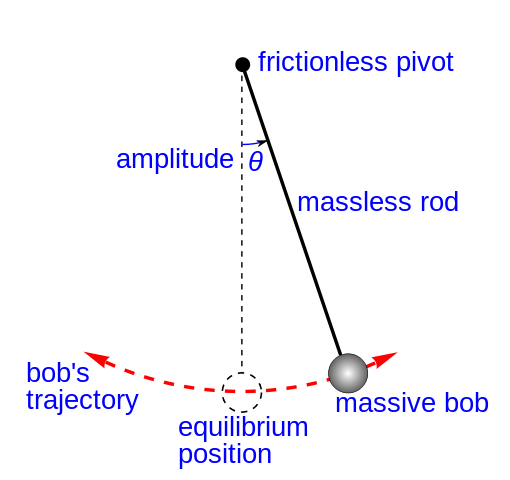
\includegraphics[width=9cm]{title2}
\vfill

\end{titlepage}

\tableofcontents
\chapter{Introduction}
Simple Harmonic Motion appears in many regions of physics, as it serves for a useful mathematical model, to describe a variety of motions. Last year, we had chosen this topic and performed an experiment to observe the phenonmenon of beats, in a dual pendulum system, where one pendulum held a light source, and the other held a convex lens. The objective of the experiment was to obtain a sharp image of the light source on a screen, during the simultaneous oscilatory motion of both the pendulums. The success of this experiment, and its interesting observations, prompted us to re-take the SHM topic this year, and perform another experiment on the same.\\ \\
SHM describes the motion of a body to be sinusoidal in time, and this aspect of it often leads it to be used as an approximation of several motions in mechanics. One such example is the motion of a Simple Pendulum. The motion of a pendulum is assumed to follow an SHM for small amplitudes. The objective of this experiment is to determine how accurate this assumption is for bigger amplitudes. We do the same by predicting the angle of release of a body in pendulum motion, whose string has been cut during its oscillatory motion.

%%% Local Variables:
%%% mode: latex
%%% TeX-master: "../experiment"
%%% End:

\chapter{Experiments}
\section{Error in Small Angle Approximation of a Pendulum}
\subsection{Aim}
\begin{enumerate}[(a)]
\item To predict the angle of release of pendulum projectile by measuring range of the projectile.
\item To use the results of (a) to compare the predictions of SAA with a more accurate analysis from energy conservation in the system. 
\end{enumerate}
\subsection{Materials Required}
Metallic bob, Thread, Iron Stand, Protractor, Metre Scale, Scissors
\subsection{Theory}
\emph{Simple harmonic motion} is a type of periodic motion where the restoring force is directly proportional to the displacement and acts in the direction opposite to that of displacement. The restoring force is given by:
\[
  \mathbf{F}=-kx
\]
where $\mathbf{F}$ is the restoring force, $k$ is a constant, and $x$ is the displacement from the equillibrium position.

A pendulum is a weight suspended from a frictionless pivot so that it can swing freely. For a pendulum to act as an SHM oscillator, the force on the weight must be proportional to the displacement of the weight from the equillibrium position. But from \textit{fig.1} it can be clearly seen that the magnitude of the restoring torque of $mg$ is given by:
\[
  |\bm{\Gamma}|=-mgl\sin\theta
\]
It is clearly seen that the restoring torque is not directly proportional to the angular displacement, which means that the pendulum is not an SHM oscillator. But for small values of $\theta$, $\sin\theta$ is approximately equal to $\theta$, and thus for this case alone does the pendulum act as an SHM. The displacement of the weight for small angles can thus be given by:
\[
  \theta=\phi\cos\omega t
\]
where $\phi$ is the amplitude (in this case, the initial \emph{angle of release} of the pendulum),$\omega$ is the angular frequency, and $t$ is a time instant.

Differentiating with respect to time, we obtain:
\[
  \frac{\dd{\theta}}{\dd{t}}=\vec{\omega}=\phi\omega\cos\omega t
\]
and since the tangential velocity $v=r\omega$, in this case,
\[
  \boxed{v=l\phi\omega\cos\omega t} \numberthis \label{eqn}
\]
where $l$ is the length of the pendulum.

We can avoid the above approximations, by considering the $\sin\theta$ term and adopting another approach through calculus to find $v$. From \emph{fig.1}, the tangential acceleration of the weight is given by:
  \[a_t=-g\sin\theta\]
We know that $a_t=\frac{\dd{v}}{\dd{t}}$, thus,
  \[\frac{\dd{v}}{\dd{s}}\frac{\dd{s}}{\dd{t}}=-g\sin\theta\]
Furthermore, $\frac{\dd{s}}{\dd{t}}=v$,from which we obtain
  \[v\dd{v}=-g\sin\theta\dd{s}\]
Integrating on both sides,
  \begin{align*}
    &\int_0^v v\dd{v} = -\int_\phi^\theta gl\sin\theta\dd{\theta} &&\text{($\because\dd{s}=l\dd{\theta}$)}\\
   \implies &\frac{v^2}{2} = gl[ \cos\theta ]^\theta_\phi = gl[\cos\theta - \cos\phi]\\
   \implies &\boxed{v=\sqrt{2gl[ \cos\theta - \cos\phi ]}} \numberthis \label{eqn} 
  \end{align*}
Which is the general expression for the velocity of the weight in a pendulum as a function of $\theta$ without any \emph{small angle approximations}.

[\emph{To be continued..}]
\subsection{Procedure}
\begin{enumerate}
\item Create a pendulum by tying a cork to one end of a string, and a bob to the other end, and then attaching the cork to an iron stand.
\item Measure the \emph{length of the pendulum} (length from the point of suspension to the centre of the bob) and the length from the centre of the bob to the ground (when bob is at equllibrium), and note them down.
  \item Put a metre scale on the ground, aligning its zero with the bob's equillibrium position when seen from above the bob. Ensure the metre scale is parallel to the pendulum motion of the bob.
\item Hold the bob away from its equillibrium position, and meausure the angle of release $\phi$ as shown in \emph{fig.2}.
\item Release the bob and cut the string with a pair of scissors at any arbitrary time in the pendulum's motion.
\item Note the range $R$ where the bob falls on the metre scale.
\item Repeat steps 4-6 for 4 more different values of the initial angle $\phi$.
\end{enumerate}
\subsection{Observations}
[Table to be planned out]
\subsection{Result}
[To be planned out]
\subsection{Precautions}
\begin{enumerate}
\item Ensure that the string has no knots, and its weight is negligible.
\item Do not cut the pendulum too late, as the amplitude might get damped, due to energy loss from friction in the air.
\item Ensure that string is cut carefully, without disturbing the oscillations in the cutting process.
\item Avoid any parallax while measuring angles/lengths.
\end{enumerate}




  

                                                                           
%%% Local Variables:
%%% mode: latex
%%% TeX-master: "../experiment"
%%% End:

\end{document}